\chapter{Garment Depth Map Clustering}
\label{garment_clustering}

This chapter explains in detail the gament analysis that our algorithm performs to the garment data previously segmented. The contour of the garment is extracted, and a Watershed segmentation algorithm is applied to find the different overlapped patches.

\section{Depth image preprocessing}
\label{depth_image_preprocessing}

Once the garment mask has been calculated, it is applied to the depth image of the garment to discard the information related to the table. The garment depth data is then normalized to prepare it for posterior analysis steps.


\section{Watershed segmentation}

Watershed\footnote{\url{http://scikit-image.org/docs/dev/auto_examples/plot_watershed.html}} is a segmentation algorithm that considers a greyscale image as a topological surface where high intensity pixels correspond to peaks and hills, and low intensity pixels are equivalent to valleys. The algorithm fills the surface pouring water at each isolated valley. As the water level rises, the water from different sources will start to merge. To prevent them from merging, the algorithm constructs barriers at the merging regions, and continues this process of adding water and building barriers until all the peaks have been flooded. The resulting barriers are the segmentation result, where each region enclosed correspond to a segmented item.

\begin{figure}[thpb]
    \centering
    
\includegraphics[width=0.7
    \textwidth]{figures/placeholder2.png}
    \caption{\comment{(Here it would be great to add a figure of the example, such as opencv's coins)}}
    \label{fig:watershed_example}
\end{figure}


In the context of this work, the Watershed segmentation algorithm is applied to the depth image of the garment to locate the different parts that are overlapping each other. This regions are related to folded parts, that rest on top of other parts of the garment. 

As in practise flooding using local minima as makers leads to over- segmentation, an enhanced version of this algorithm allows the user to specify other criteria for selecting the seed points. The gradient of the greyscale depth-image was calculated for this work, and regions where the gradient has a low value were selected. These regions correspond to homogeneous and continous regions, which are good candidates to be used as markers.

To prepare it for the Watershed segmentation, the depth image was normalized and converted to a greyscale image. A denoising step was also performed, using a total variation filter \comment{(ref chambolle)}, to produce a smoother image, while maintaining the edges sharp. The total variation filter works by minimizing the integral of the norm of the image gradient. As a result of this filter, piecewise-constant images (``cartoon-like'' images) are obtained.

The different garment regions obtained with watershed were labeled and used as input for the next step. Figure \ref{fig:watershed_labels} shows the result of this process.

\begin{figure}[thpb]
    \centering
    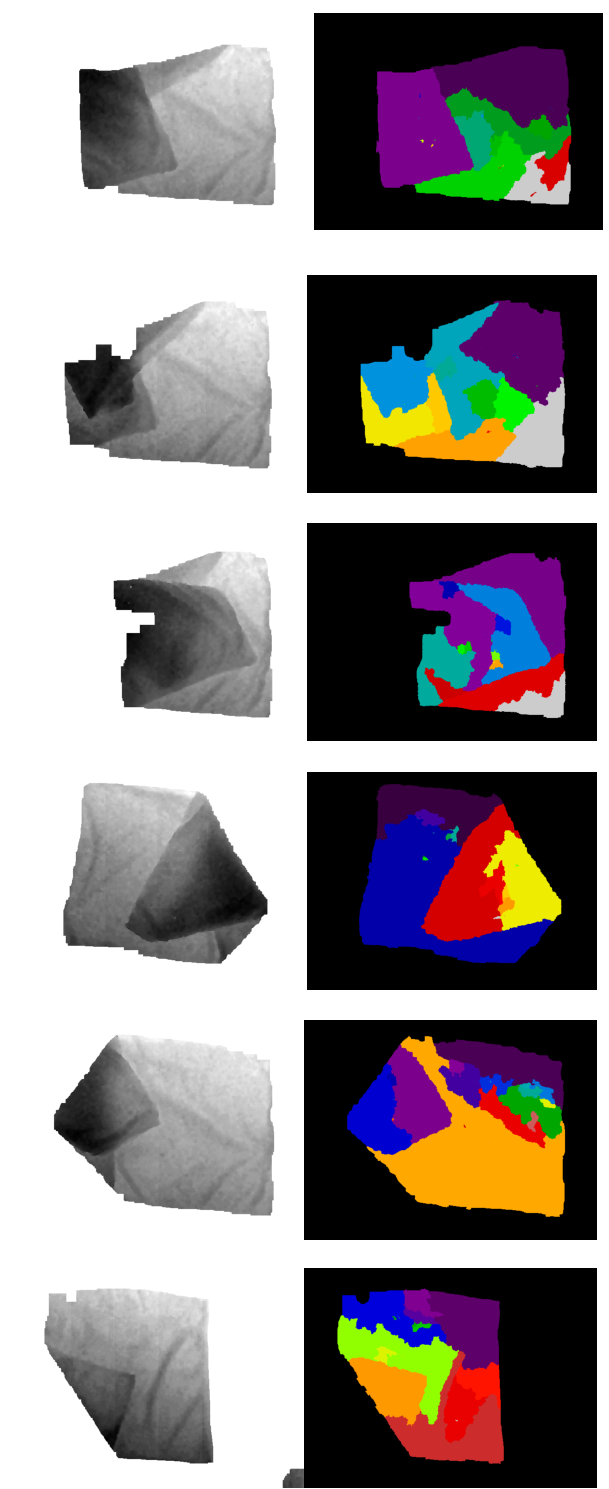
\includegraphics[width=0.38\textwidth]{figures/colour_garment.pdf}
    \caption{On the left side, the grayscale images are shown. The grey level is related to the height of the point as detected by the RGB-D sensor. On the right side, the labeled image returned by watershed algorithm is presented, where each color represents a region of similar height.}
    \label{fig:watershed_labels}
\end{figure}